\title{18. Tečny k funkcím a kuželosečkám}
\author{Jakub Švagr}
\date{2.5.2025}

\maketitle

\section{Tečna}
Tečna je přímka, která má k dané funkci nebo kuželosečce v určitém bodě stejný směrový vektor (směrnici), jako ta funkce nebo kuželosečka. Tečna leží vně (venku) funkce, až na jeden společný bod, který sdílí s funkcí.

\subsection{Normála}
Normála je přímka kolmá na tečnu, která prochází bodem dotyku. Rovnice normály se získá z rovnice tečny změnou směrnice na její zápornou převrácenou hodnotu.
\[
Ax + By + C = 0
\]

\begin{itemize}
  \item \( A, B, C \) jsou reálné konstanty
  \item pokud \( B \neq 0 \), můžeme tvar převést do směrnicového
  \item směrnice přímky je potom \( k = -\frac{A}{B} \)
\end{itemize}

\subsection{Směrnice}
Směrnice přímky je tangens úhlu, který daná přímka svírá s kladnou poloosou x.
\[
y = kx + q
\]
\begin{itemize}
  \item \( k \) je směrnice přímky – určuje její sklon přímky,
  \item \( q \) je absolutní člen – určuje průsečík přímky s osou \( y \)
\end{itemize}

\subsection{Jak na to?}

\subsubsection{Tečna k funkci}
U funkcí hledáme tečnu pomocí derivace. Derivace funkce v bodě udává hodnotu směrnice tečny.
\begin{enumerate}
\item Máme funkci \( f(x) = \frac{2x + 1}{x^2} \), chceme najít rovnici tečny v bodě \( T[-2; ?] \).

\item Nejdříve spočítáme funkční hodnotu tím, že za x dosadíme -2:

\[
f(-2) = \frac{2 \cdot (-2) + 1}{(-2)^2} = \frac{-4 + 1}{4} = \frac{-3}{4}
\]

Bod dotyku je tedy \( T[-2; -\frac{3}{4}] \).

\item Nyní funkci zderivujeme, tím získáme:

\[
f'(x) = \frac{2x^2-(2x+1)2x}{x^4}= \frac{2x(x-(2x+1))}{x^4}= \frac{2(-x-1)}{x^3}= \frac{-2(1+x)}{x^3}
\]

\item Dosadíme \( x = -2 \) do zderivované funkce:

\[
f'(x) = -\frac{2([-2]+1)}{(-2)^3} = -\frac{-2}{-8} = -\frac{1}{4}
\]

\item Tečna má tedy směrnici \( -\frac{1}{4} \), bodem \( T[-2; -\frac{3}{4}] \) vede tečna s rovnicí:
\[
y = -\frac{1}{4}x +c 
\]
dosadíme za souřadnice x a y
\[
-\frac{3}{4} = -\frac{1}{4}(-2) +c 
\]
\[
-\frac{3}{4} = \frac{1}{2} +c 
\]\[
-\frac{5}{4} =c 
\]
dosadíme vypočítané $c$ do rovnice a máme rovnici tečny funkce v daném bodě
\[
y = -\frac{x}{4} - \frac{5}{4} 
\]
\end{enumerate}
    \begin{figure}[h]
        \centering
        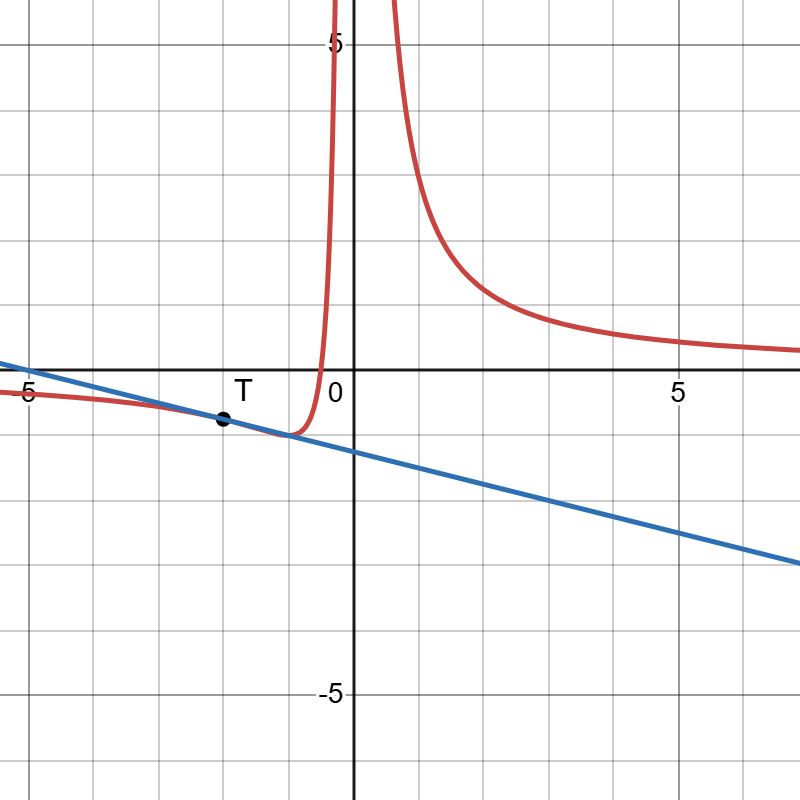
\includegraphics[width=0.5\linewidth]{img/17_Tecna_k_funkci.png}
        \caption{Tečna k funkci \(f(x) = \frac{2x + 1}{x^2}\)}
        \label{fig:enter-label}
    \end{figure}
\subsubsection{Tečna ke kuželosečce}
U kuželoseček hledáme tečnu pomocí soustavy rovnic a diskriminantu. Pokud dosadíme rovnici přímky do rovnice kuželosečky, vznikne kvadratická rovnice. Tečna nastane tehdy, pokud má tato rovnice právě jedno řešení, tedy diskriminant je roven nule (neplatí pro parabolu, kdy sečna může mít jeden společný bod s kuželosečkou, pokud je rovnoběžná s osou).

\begin{enumerate}
\item Máme rovnici paraboly a přímku p, počítá se to jako soustava rovnic:
\[
P: y^2 - 16x - 4y - 12 = 0
\]
\[
p: x - y + c = 0
\]
\item Vyjádřeme si to, co pro nás bude lehčí, v tomto případě je to celkem jedno, ale zvolil jsem \(x\).
\[x = y - c\]

\item Dosadíme \( x \) z přímky do rovnice kuželosečky:

\[
y^2 - 16(y - c) - 4y - 12 = 0
\]
\[
y^2 - 16y + 16c - 4y -12 = 0
\]
\[
y^2 - 20y + 16c - 12 = 0
\]

\item Aby to byla tečna, kvadratická rovnice musí mít právě jedno řešení, tedy diskriminant \( D \) musí být roven nule:

\[
D = (-20)^2 - 4 \cdot 1 \cdot (16c - 12) = 400 - 64c + 48 = 448 - 64c
\]

\[
448 - 64c = 0 
\]
\[
c = \frac{448}{64} = 7
\]

\item Hodnota \( c = 7 \), naše tečna je tedy \( x - y + 7 = 0 \).
\end{enumerate}
\begin{figure}[h]
    \centering
    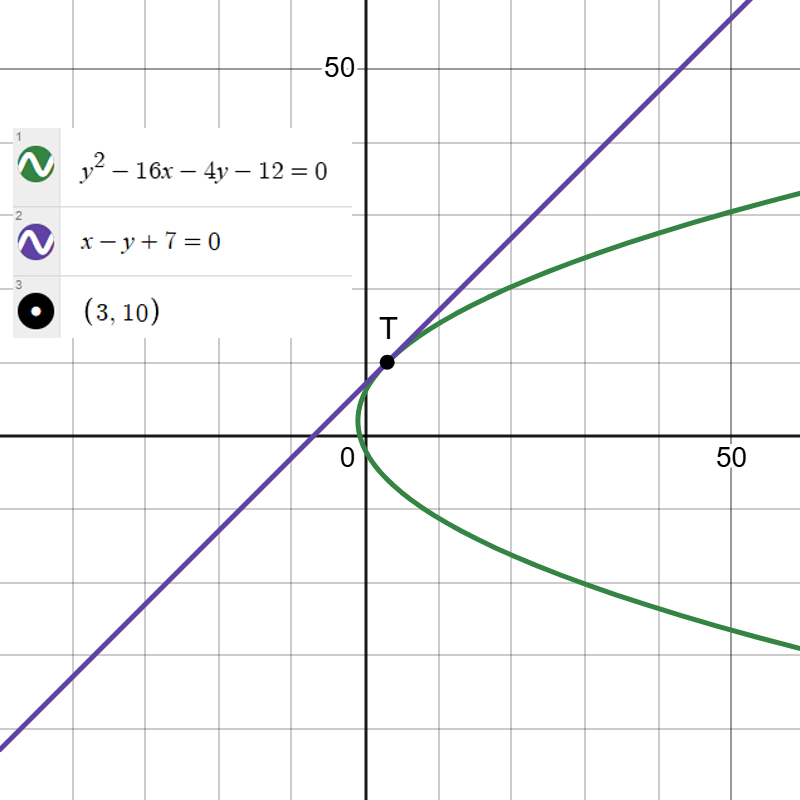
\includegraphics[width=0.3\linewidth]{img/17_Tecna_k_parabole.png}
    \caption{Tečna k parabole \(P: y^2 - 16x - 4y - 12 = 0\)}
    \label{fig:enter-label}
\end{figure}
\textbf{POZOR!} U paraboly nestačí, aby diskriminant byl nulový, protože se může stát, že přímka s kuželosečkou má právě jeden společný bod, ale není tečnou, ale sečnou. Toto se stane pokud je naše přímka kolmá na řídící přímku paraboly.
\subsubsection{Tečna u kuželoseček pokud máme bod doteku}
Existuje i jiná cesta, jak získat tečnu ke kuželosečce, a to pomocí vzorečků, zde je tabulka:
\begin{table}[h]
    \centering
    \begin{tabular}{|c|c|c|}
        \hline
        \textbf{Kuželosečka} & \textbf{Středová rovnice kuželosečky} & \textbf{Rovnice tečny v bodě $[x_0, y_0]$} \\ \hline
        Kružnice & $(x - m)^2 + (y - n)^2 = r^2$ & $(x_0 - m)(x - m) + (y_0 - n)(y - n) = r^2$ \\ \hline
        Elipsa & $\frac{(x - m)^2}{a^2} + \frac{(y - n)^2}{b^2} = 1$ & $\frac{(x_0 - m)(x - m)}{a^2} + \frac{(y_0 - n)(y - n)}{b^2} = 1$ \\ \hline
        Parabola & $(x - m)^2 = 2p(y - n)$ & $((y_0 - n)(y - n)=2p[(x - m)+(x_0 - m)])$ \\ \hline
        Hyperbola & $\frac{(x - m)^2}{a^2} - \frac{(y - n)^2}{b^2} = 1$ & $\frac{(x_0 - m)(x - m)}{a^2} - \frac{(y_0 - n)(y - n)}{b^2} = 1$ \\ \hline
    \end{tabular}
    \caption{Přehled rovnic kuželoseček a jejich tečen}
    \label{tab:kuželosečky}
\end{table}
\begin{enumerate}
\item Zde stačí pouze do rovnice dát souřadnice bodu doteku. Vezměme si rovnici paraboly. Toto je, mimochodem, ta stejná parabola, přepsaná v do středového útvaru.
\[
(y - 2)^2=16(x+1)
\]

\item Určeme si souřadnice středu a parametr, pro přehlednost:
\[
(y - 2)^2 = 16(x+1), 
m=-1,\;n=2,\;2p=16\;\Longrightarrow\;p=8
\]
\item Vezměme si rovnici z tabulky:
\[
(y_0 - n)(y - n) = p\bigl[(x-m)+(x_0-m)\bigr]
\]
\item Dosadíme do ní naše hodnoty:
\[
(10-2)(y-2) = 8\bigl[(x+1)+(3+1)\bigr]
\]
\item Pak to upravíme a dostaneme toto:
\[
8(y-2) = 8(x+5)
\]
\[
y-2 = x+5
\]
\[
x - y + 7 = 0
\]
\end{enumerate}